% Introdução — versão 2, 01/11/2026.
% Preserva o padrão de títulos do template UENP utilizado no projeto.
% Bibliografias: referencias_tcc.bib, referencias_fundamentacao.bib
% e referencias_introducao_v2.bib. Instruções em LEIA_ME_INTRODUCAO_V2.md.
\begingroup
\justifying
\setlength{\parindent}{1.25cm}
\setlength{\parskip}{0pt}
\onehalfspacing
\setlength{\emergencystretch}{1em}

\phantomsection
\addcontentsline{toc}{section}{1 INTRODUÇÃO}
\noindent\textbf{1 INTRODUÇÃO}\par
\vspace{\baselineskip}

Antes que uma cirurgia seja realizada, os instrumentos necessários precisam estar disponíveis, organizados e conferidos. Após o uso, esses materiais retornam a um fluxo de recebimento, limpeza, preparo e esterilização que permite sua utilização em novos procedimentos. Nesse percurso, reconhecer cada peça e verificar as quantidades são tarefas que conectam o trabalho de diferentes profissionais. No Hospital Universitário da Universidade Estadual de Londrina (HU-UEL), o estudo de \textcite{moreto2025} descreve conferências tanto na recepção do material utilizado quanto no preparo dos conjuntos que serão encaminhados à esterilização.

Esses conjuntos são frequentemente organizados em caixas cirúrgicas: recipientes que reúnem instrumentos selecionados para atender a determinado procedimento ou especialidade. Cada caixa possui uma composição de tipos e quantidades definida pelo serviço. Assim, uma caixa destinada a uma cirurgia cardíaca pode reunir instrumentos diferentes daqueles utilizados em neurocirurgia ou em uma apendicectomia, procedimento de retirada do apêndice. A caixa de apendicectomia adotada como referência nesta pesquisa delimita os objetos de interesse, entre eles pinças, tesouras e afastadores. Essa delimitação permite estudar um conjunto concreto de materiais, associado a uma necessidade hospitalar, em vez de tentar reconhecer indiscriminadamente todos os instrumentos existentes.

A conferência desses materiais tem importância tanto para a organização do serviço quanto para a segurança do cuidado. Durante a cirurgia, a contagem de instrumentos, compressas e agulhas integra as medidas recomendadas pela Organização Mundial da Saúde (OMS) para prevenir que materiais permaneçam inadvertidamente no paciente \parencite{oms2009}. No Brasil, a segurança cirúrgica também faz parte das ações do Programa Nacional de Segurança do Paciente \parencite{brasil2014}. A conferência realizada no processamento dos instrumentos e a contagem durante a operação, contudo, correspondem a momentos diferentes. O presente estudo se concentra no primeiro contexto: o apoio à identificação e à contagem de instrumentos fora do paciente, a partir de fotografias.

A importância dessa conferência também é evidenciada pelos casos de retenção não intencional de materiais. Em um estudo realizado em hospitais de Massachusetts, nos Estados Unidos, \textcite{gawande2003} identificaram uma ocorrência de retenção a cada 8.801 a 18.760 operações hospitalares no período de 1990 a 2000. Entre os casos de retenção em que a contagem havia sido realizada, 88\% apresentavam registro de contagem correta. Esses dados históricos abrangem compressas e instrumentos e não representam uma estimativa para o HU-UEL. Eles mostram, contudo, que a concordância numérica, isoladamente, não garante a ausência de materiais retidos. Por isso, a contagem automática é investigada como recurso de apoio à conferência, sem substituir os demais procedimentos de segurança.

Esse contexto envolve o Centro de Material e Esterilização (CME), setor responsável pelo processamento dos materiais utilizados na assistência. No fluxo descrito por \textcite{moreto2025}, o expurgo recebe os instrumentos utilizados, que passam pela conferência e pela limpeza; na área de preparo, outra conferência acompanha a organização e o fechamento das caixas. O registro individual das peças nesses pontos evidencia uma tarefa repetitiva que motiva a investigação de recursos de apoio. Nesta pesquisa, a aplicação é pretendida em ambos os ambientes, e as fotografias hospitalares foram obtidas tanto no expurgo quanto na área de preparo. A questão é saber se um computador pode extrair de uma imagem informações suficientemente confiáveis sobre quais instrumentos estão presentes e em que quantidade.

A área da computação que estuda a obtenção de informações a partir de imagens é chamada de visão computacional. Suas aplicações incluem o reconhecimento de objetos e a análise de imagens médicas, entre outras tarefas em que informações visuais precisam ser interpretadas. Uma das abordagens utilizadas é o aprendizado de máquina: em vez de escrever uma regra para cada possível aparência de um objeto, são apresentados exemplos a um modelo computacional, que ajusta seu funcionamento para reconhecer padrões. As redes neurais são modelos formados por operações interligadas, com valores ajustáveis durante esse aprendizado. Quando utilizam múltiplas camadas de processamento para aprender representações dos dados, integram o campo do aprendizado profundo \parencite{goodfellow2016}.

Para a conferência de instrumentos, não basta reconhecer que uma fotografia contém uma pinça. É necessário localizar cada objeto individual, inclusive quando vários aparecem juntos. Essa tarefa é chamada de detecção de objetos. Uma forma usual de apresentar seu resultado é desenhar um retângulo ao redor de cada objeto e associá-lo a uma classe, isto é, à categoria que o identifica. O retângulo recebe o nome de caixa delimitadora. Quando cada instrumento é localizado uma única vez e recebe a identificação correta, essas detecções podem ser somadas para obter a quantidade total e a quantidade por categoria.

% A figura e sua chamada só aparecem quando a fotografia revisada estiver disponível.
% Inserir imagem real anotada, nunca uma saída fictícia apresentada como predição.
\IfFileExists{figuras/exemplo_caixa_delimitadora_hu.png}{%
A Figura~\ref{fig:intro-caixa-delimitadora} exemplifica essa representação em uma fotografia do conjunto hospitalar. A marcação foi realizada para indicar o objeto de interesse e sua categoria.

\begin{figure}[htbp]
\centering
\caption{Exemplo de instrumento identificado por uma caixa delimitadora}
\label{fig:intro-caixa-delimitadora}
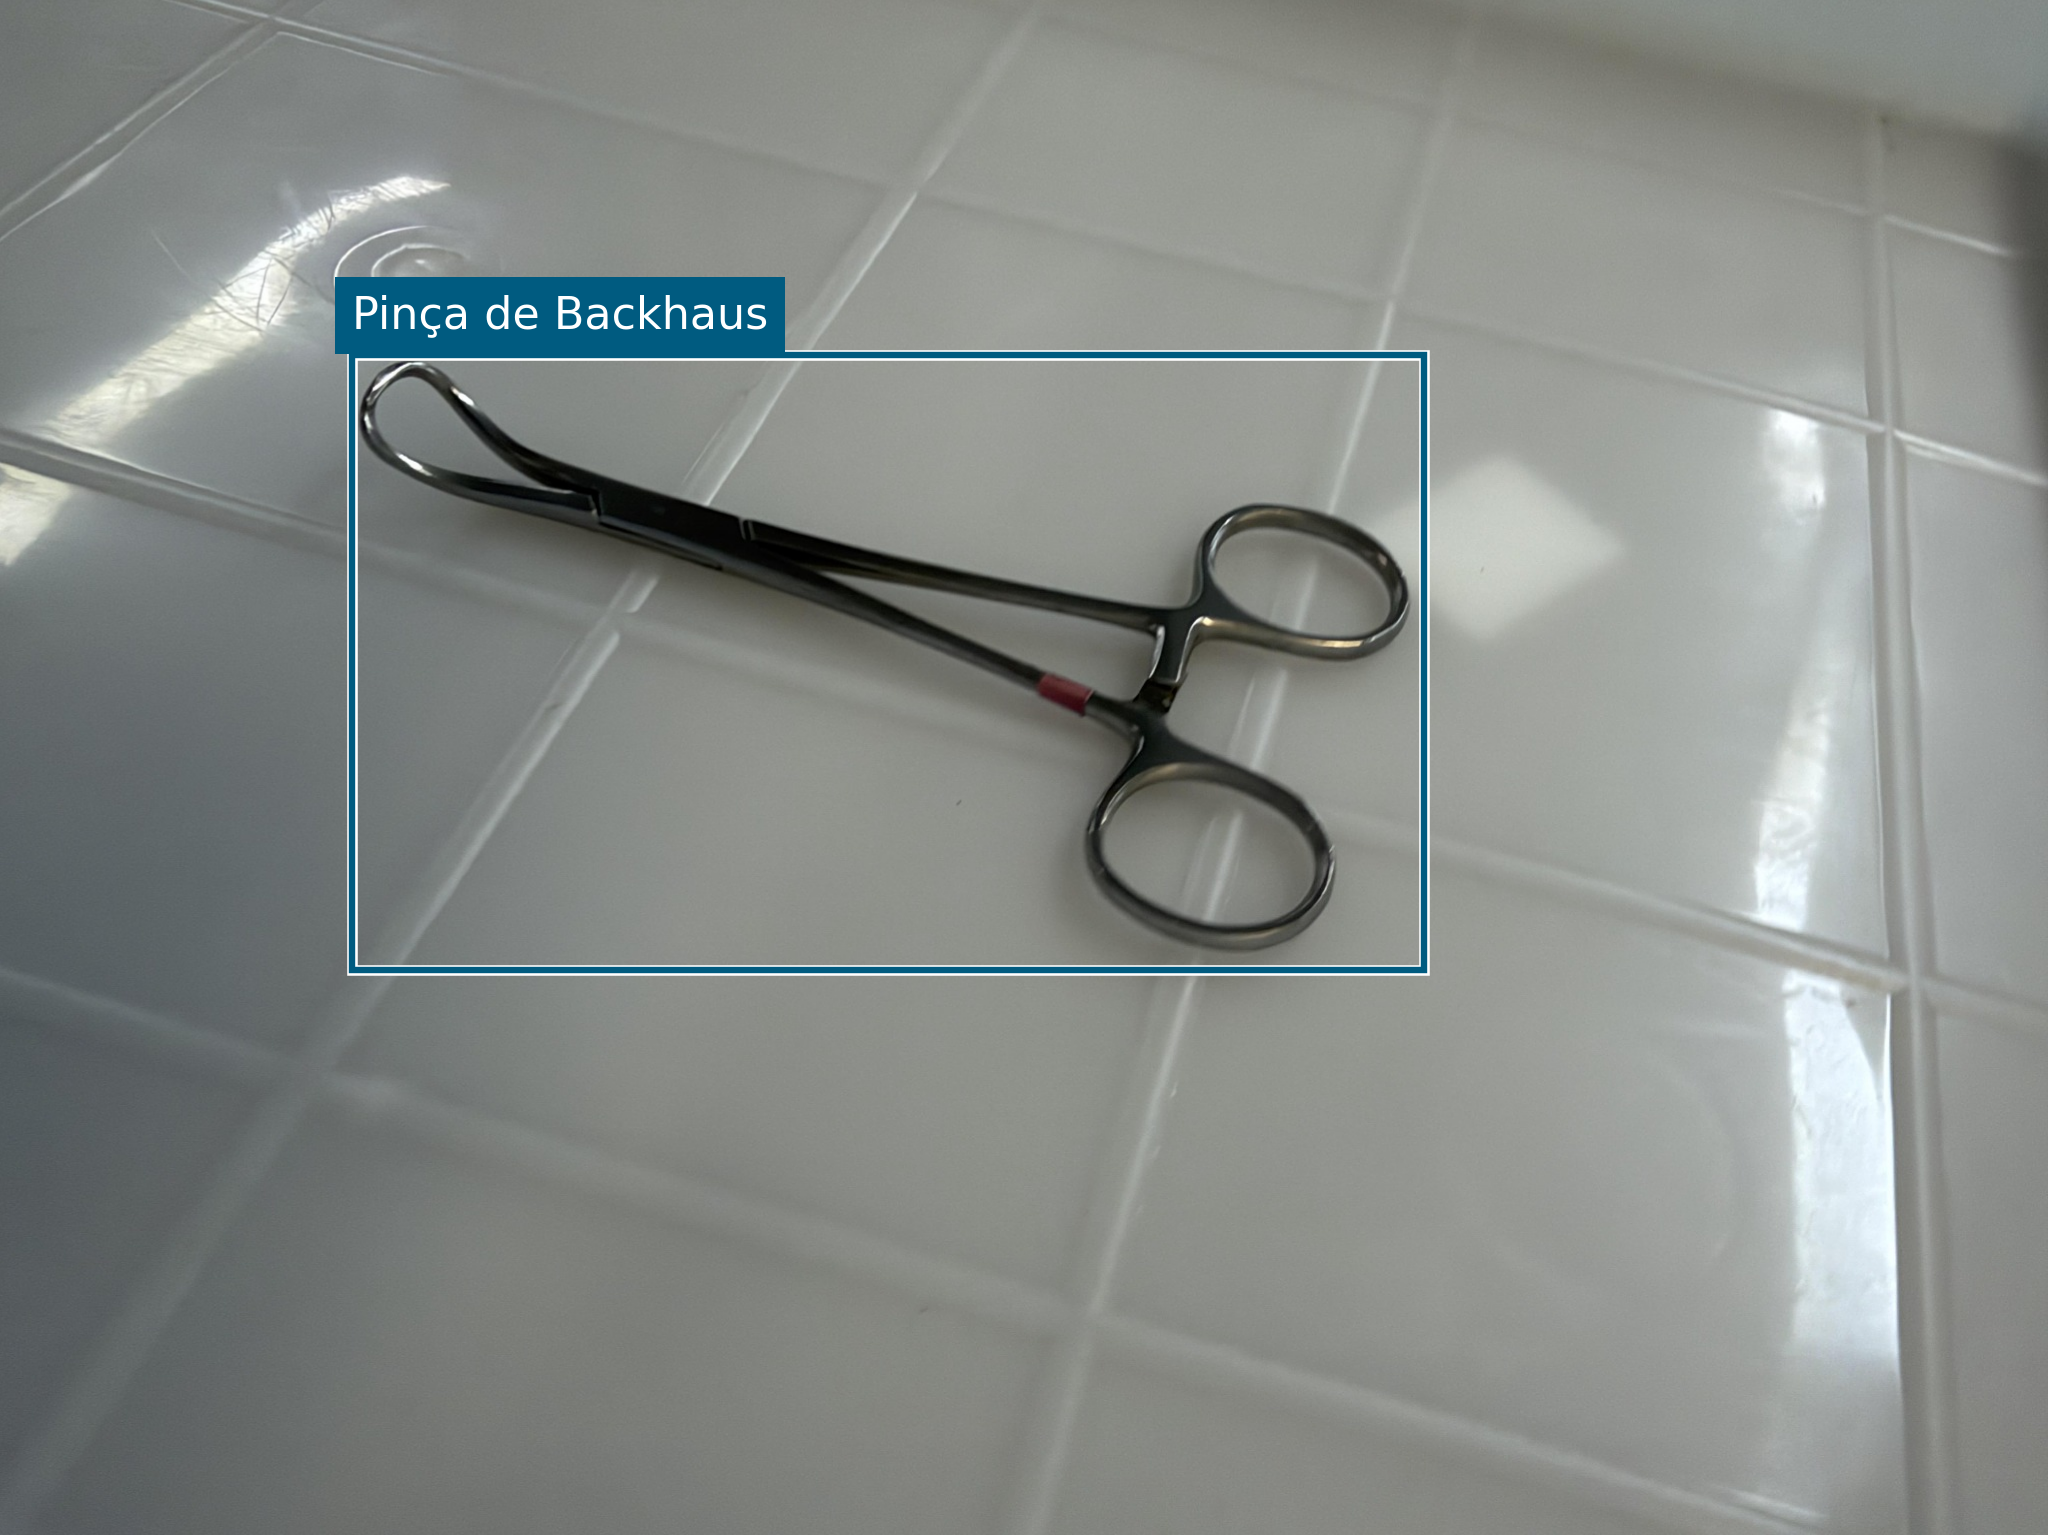
\includegraphics[width=0.72\linewidth,height=0.30\textheight,keepaspectratio]{figuras/exemplo_caixa_delimitadora_hu.png}
\par\smallskip
{\footnotesize Fonte: elaboração própria, a partir de fotografia do conjunto HU-UEL (2026).\par}
\end{figure}
}{}

Para aprender a realizar essa tarefa, o modelo recebe imagens acompanhadas de marcações que indicam a posição e a classe dos objetos. Essas marcações são as anotações de referência: exemplos revisados que orientam o aprendizado e permitem, posteriormente, comparar a resposta do modelo com os objetos efetivamente presentes na imagem. A qualidade desse material importa porque uma caixa mal posicionada, uma classe incorreta ou um instrumento não marcado pode comprometer o aprendizado e a avaliação. Por isso, preparar uma base de imagens envolve selecionar os exemplos, conferir as marcações e organizar nomes e categorias antes do treinamento.

Entre os modelos desenvolvidos para detectar objetos estão o Faster R-CNN e os modelos da família \textit{You Only Look Once} (YOLO). No Faster R-CNN, o processamento inclui a proposta de regiões que podem conter objetos e a análise dessas regiões para classificá-los e ajustar sua localização \parencite{ren2015faster}. A proposta original do YOLO reúne a estimativa das posições e das classes em um processamento da imagem completa, com ênfase na rapidez da detecção \parencite{redmon2016}. Essas abordagens oferecem caminhos distintos para o mesmo problema; a escolha entre elas depende da aplicação, dos dados e dos recursos disponíveis.

Neste estudo, foi selecionada a família YOLO por combinar a localização e a identificação dos objetos em uma solução que permite construir a contagem a partir das detecções. A escolha também encontra apoio em pesquisas sobre instrumentos cirúrgicos, como as de \textcite{ran2023} e \textcite{jiang2023}, que investigaram adaptações de versões anteriores dessa família. Seus resultados motivam a investigação, mas não antecipam o desempenho nas fotografias utilizadas aqui. O modelo adotado é o YOLO26n, variante compacta da família YOLO26. Essa família disponibiliza variantes de diferentes tamanhos, identificadas por n, s, m, l e x, com diferentes necessidades de processamento \parencite{ultralyticsYOLO26intro}. A escolha da variante n considerou os recursos computacionais disponíveis e a possibilidade de avaliar uma solução de menor porte, mantendo a qualidade das detecções e das contagens como questões a serem examinadas experimentalmente.

Essa avaliação exige separar o aprendizado da verificação de seus resultados. As imagens de treinamento são utilizadas para ajustar o modelo; as de validação permitem acompanhar o aprendizado e orientar escolhas de configuração; e as de teste são reservadas para avaliar o desempenho após essas escolhas. Também é necessário preparar as imagens para a entrada da rede. Fotografias de dimensões diferentes são redimensionadas e, quando necessário, recebem preenchimento nas bordas para se adequar ao tamanho de processamento adotado. Esse procedimento facilita a execução computacional, mas pode reduzir detalhes relevantes para distinguir instrumentos semelhantes. As decisões de preparação e avaliação, portanto, fazem parte do problema investigado, e não apenas da execução do programa.

\vspace{\baselineskip}
\phantomsection
\addcontentsline{toc}{subsection}{1.1 Problema de pesquisa e justificativa}
\noindent\textbf{1.1 Problema de pesquisa e justificativa}\par
\vspace{\baselineskip}

A possibilidade de contar instrumentos por imagens é atraente, mas seu uso depende de reconhecer os objetos apesar das variações presentes nas fotografias. Instrumentos metálicos podem produzir reflexos; peças diferentes podem ter formatos semelhantes; e um objeto pode esconder parte de outro. Essas condições dificultam a localização e a identificação, como discutido nos estudos de \textcite{ran2023} e \textcite{jiang2023}. Por isso, a existência de um detector capaz de reconhecer objetos em outras aplicações não é suficiente para concluir que ele atenderá à conferência pretendida no hospital.

A pergunta que orienta esta pesquisa é: em que medida um modelo da família YOLO é tecnicamente viável para identificar e contar instrumentos selecionados da caixa de apendicectomia, nas condições representadas pelas fotografias de avaliação, visando ao apoio à conferência no expurgo e no preparo de caixas cirúrgicas?

Neste contexto, avaliar a viabilidade significa examinar a qualidade das detecções, os erros de contagem, os tempos de treinamento e de processamento das imagens e as situações em que o modelo apresenta dificuldades. Acertar somente o total de objetos não é suficiente. Em uma imagem com dois instrumentos, por exemplo, o modelo pode deixar de reconhecer um deles e marcar indevidamente outra região, produzindo duas detecções apesar do erro. Também pode localizar ambos e trocar suas classes. A análise precisa, portanto, considerar tanto o total quanto a identificação e a localização dos objetos que deram origem à contagem. Os indicadores e os procedimentos utilizados para essa análise são apresentados na metodologia.

A contribuição pretendida é oferecer evidências sobre as possibilidades e os limites dessa abordagem em um conjunto relacionado à rotina do HU-UEL. Para isso, foram reunidas imagens de bases disponíveis na internet e fotografias hospitalares, com revisão dos objetos e de suas anotações. A combinação dessas fontes fornece exemplos para o treinamento, enquanto a avaliação deve mostrar até que ponto o modelo consegue lidar com imagens que não foram utilizadas para ajustá-lo. O estudo trata a contagem automática como um possível recurso de apoio à conferência profissional, sem pressupor que o desempenho em fotografias demonstre, por si só, redução de acidentes ou prontidão para uso assistencial.

\vspace{\baselineskip}
\phantomsection
\addcontentsline{toc}{subsection}{1.2 Objetivos}
\noindent\textbf{1.2 Objetivos}\par
\vspace{\baselineskip}

O objetivo geral é avaliar a viabilidade técnica da detecção e da contagem automática de instrumentos selecionados da caixa de apendicectomia, agrupados em sete categorias gerais, por meio do modelo YOLO26n, visando ao apoio à conferência no expurgo e no preparo de caixas cirúrgicas.

Para alcançar esse objetivo, foram definidos os seguintes objetivos específicos:
\begin{list}{\alph{enumi})}{\usecounter{enumi}\setlength{\leftmargin}{1.25cm}\setlength{\labelsep}{0.5em}\setlength{\itemsep}{0pt}\setlength{\parsep}{0pt}\setlength{\topsep}{0pt}}
\item organizar e revisar as imagens da internet e do HU-UEL, padronizando as categorias e as anotações dos objetos;
\item preparar os conjuntos de treinamento, validação e teste, com controle de duplicatas e agrupamento das imagens relacionadas identificadas;
\item treinar um modelo YOLO para localizar e identificar os instrumentos nas categorias gerais adotadas;
\item avaliar a detecção e a contagem, considerando os resultados totais, os resultados por categoria e a frequência de imagens com contagem correta;
\item analisar os erros e os tempos de treinamento e de processamento por imagem, identificando condições favoráveis e limitações para a aplicação pretendida.
\end{list}

\vspace{\baselineskip}
\phantomsection
\addcontentsline{toc}{subsection}{1.3 Delimitação do estudo}
\noindent\textbf{1.3 Delimitação do estudo}\par
\vspace{\baselineskip}

O experimento utiliza fotografias estáticas e sete categorias gerais: pinças, tesouras, afastadores, porta-agulhas, cabos de bisturi, bicos de aspiração e cúpulas. As cúpulas são recipientes que também integram a contagem dos objetos de interesse. O foco é localizar os objetos e estimar suas quantidades, sem distinguir todos os tipos de instrumentos pertencentes a uma mesma categoria. A correspondência entre os instrumentos selecionados e as categorias utilizadas no treinamento é apresentada na metodologia. Diferenças de tamanho não originam classes distintas.

O agrupamento reúne exemplos de diferentes instrumentos sob um número menor de rótulos e delimita uma tarefa compatível com o objetivo de avaliar a contagem. Essa organização foi considerada pertinente diante da distribuição desigual dos exemplos disponíveis. Entretanto, a pesquisa não compara categorias gerais e específicas e, portanto, não permite afirmar que o agrupamento produziu desempenho superior. Também permanece necessária a análise por categoria, pois reunir instrumentos diferentes não elimina a diversidade visual nem o desequilíbrio da base.

A seleção foi limitada aos objetos de interesse para os quais se obtiveram imagens adequadas. As pinças anatômicas e os cabos de bisturi estão representados somente por imagens da internet na base consolidada. Essas diferenças de cobertura devem ser consideradas ao interpretar os resultados, especialmente quando se discute a aplicação no ambiente hospitalar.

As fotografias incluem instrumentos isolados, alguns conjuntos com vários objetos e bandejas vazias. Embora tenham sido obtidas imagens nos dois ambientes de aplicação pretendidos, o estudo não equivale a uma implantação do sistema no fluxo de trabalho. A avaliação se refere aos objetos visíveis nas fotografias e às condições representadas no conjunto de teste. A conferência integral de uma caixa, o reconhecimento de materiais totalmente encobertos e a demonstração de benefícios durante o uso hospitalar exigem avaliações próprias. Dessa forma, a pesquisa busca estabelecer uma base experimental para decidir como a contagem por visão computacional pode avançar em direção à aplicação pretendida.


\endgroup
